%!TEX root = thesis.tex
\chapter{Findings} % (fold)
\label{cha:findings}

\excrumbs
{
	\textbf{Studies of software evolution have shown that the evolution of software has certain trait}
	
	Studies have shown that the evolution of software has recurring traits...
	
	- Shows repeating patterns of growth
	
	- Metrics show a skewed distribution (concentration of complex classes that are popular and become more popular over time)
	
	- But we don't yet know whether these traits are exhibited by evolving vocabulary of the source code
}

\excrumbs
{
	\textbf{Previous research of source code vocabulary:}
	
	- \cite{Abebe09a} observed that most new identifiers are composed of existing terms, rather than new terms
	
	- \cite{Antoniol07a} observed that the lexicon is more stable than the system as a whole and that changes to the lexicon are infrequent and unlikely
	
	- Their studies did not examine the distribution profiles describing how application of source code vocabulary is applied across multiple versions
	
	- No studies have investigated whether the laws of software evolution apply to vocabulary
}

\begin{itemize}
	% Growth-related questions
	\item What are the trends for growth in total size of the vocabulary across evolving software systems? Does this match findings for the growth of software systems as a whole?
	\item How stable is the growth of vocabulary across? Does the amount of growth vary from version to version and is there more volatility in earlier versions?
	
	% Distribution-related questions
	\item What is the distribution of term usage across systems?
		\begin{itemize}
			\item Is there a tendency to use particular terms with greater frequency than others? 
			\item Is the distribution profile preserved throughout evolution?
		\end{itemize}
	
	\item What kinds of terms are used with greatest frequency?
		\begin{itemize}
			\item What do the most frequently used terms refer to? Are these terms related to the domain or architectural concepts (such as idioms or design patterns)
		\end{itemize}
	\item Do the most popular terms remain the most popular or does this change as the software evolves?
\end{itemize}

\excrumbs
{
In this chapter, we:

- Address the above questions

- Use our findings to drive discussion of whether the laws of software evolution can be used to describe evolving vocabulary

- \textbf{Major outcome of research (who does it help and why)}
}

\section{Growth in Vocabulary} % (fold)
\label{sec:growth_in_vocabulary}

\subsection{Measuring Growth in Vocabulary} % (fold)
\label{sub:measuring_growth_in_vocabulary}

\crumbs{Plots of the total token count against the number of days since the initial version for each version, which is obtained through the extraction of tokens from each version of software}

\crumbs
{
\textbf{Keep this brief...can add more later to appendix}

Regression for the plot is generated to summarise the growth. From this we can determine if the growth is sub-linear, linear or super-linear
}

\crumbs{Using these plots we assess the stability of growth by observing how the versions fit this model (i.e. if the residual values closely fit the model, then the growth is stable, otherwise it is volatile)}

\crumbs{Growth of system size compared to vocabulary size is determined by plotting the system's raw size in the same manner as the vocabulary size and observing similarities in their growth patterns.}

% subsection measuring_growth_in_vocabulary (end)

\subsection{Observations of Growth} % (fold)
\label{sub:observations_of_growth}

\subsubsection{Patterns of Growth} % (fold)
\label{ssub:patterns_of_growth}

What are the trends for growth in total size of the vocabulary across evolving software systems? Does this match growth exhibited by evolving software systems as a whole?

Lehman's laws argue that evolving software systems tend to exhibit sub-linear growth rate.  This argument is based on the assumption that as software evolves its complexity increases but the overall effort towards development remains stable. Lehman's studies \cite{Lehman97a} show that increases in complexity are caused both by the size of the system (volumetric complexity) as well as the internal complexity of some of the modules.

Similarly, the sheer magnitude of a vocabulary impacts the ability of an individual to comprehend the vocabulary in its entirety [\textbf{Note: Need to cite something for this or weaken the argument}]. This would suggest that an individual will increase the size of their vocabulary so as to express themselves effectively, but that the associated volumetric complexity will eventually drive the rate of growth of the vocabulary to decrease steadily.

In this study, we investigated the growth rate of the vocabulary in order to ascertain if the sub-linear growth rate expectation extends to vocabulary.

To determine the growth rate of vocabulary, we categorised the rate of growth according to the most appropriate regression model that fit the vocabulary size across versions. These possible growth rates, along with their associated implications are highlighted in Table~\ref{tab:vocab_growth_rate_implications}. A \emph{Sub-Linear} growth rate indicates that the vocabulary is unable to sustain growth, possibly due to an inability of developers to manage the linguistic overhead that is associated with introducing a large number of new terms, a characteristic expected of a system in which the core design undergoes refinement, but is conceptually stable. Meanwhile, a \emph{Super-Linear} growth rate would suggest that the system's architecture facilitates extension, possibly through the use of a plugin architecture, allowing new terms to be introduced without impacting the core design of system and introducing complexity.

\begin{table*}[t]
\centering
\begin{tabular}{|p{.23\textwidth}|p{.72\textwidth}|}
\hline
{\bf Growth Rate} & {\bf Implications}\\
\hline
\hline
Sub-Linear
&
Developers are unable to increase the number of terms, due to the associated complexity that comes through introduction of concepts. This type of growth is expected in systems that do not easily allow extension, and are instead based around a core design that undergoes maintenance and refinement. 
\\
\hline
Super-Linear
&
Developers are able to continually increase the rate of term addition while managing the associated linguistic overhead. This type of growth is expected in systems which facilitate extension of functionality without altering the systems' core design (e.g. plug-in architectures).
\\
\hline
Linear
&
Developers are able to maintain a consistent rate of introducing new terms.
\\
\hline
\end{tabular}
\vspace{0.2cm}
\caption{The possible growth rates that may be exhibited by a vocabulary as it evolves, and the implications that are associated with these growth types.}
\label{tab:vocab_growth_rate_implications}
\vspace{-0.2cm}
\end{table*}

\begin{figure}[t]
\centering
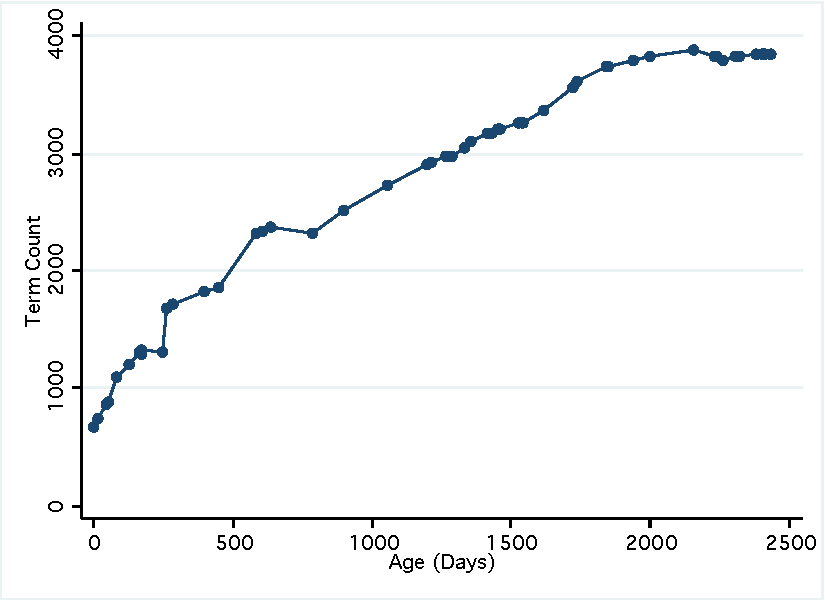
\includegraphics[width=\textwidth]{Figures/Vocab-AzureusGrowth.pdf}
\caption{The vocabulary size across the release history of Azureus, exhibiting sub-linear growth. The size of the vocabulary increases greatly throughout the earlier versions (ages 0-600), followed by a long period in which there is a steady rate of growth (ages 800-1700). Beyond this point, there is very little growth in the total size of the vocabulary for the remaining versions (ages 1800-2500)}
\label{fig:vocab-growth-azureus}
\end{figure}

% [[write a short paragraph -- few lines summarising the number of systems that showed sub-linear, linear and super linear vocabulary growth. 37 showed sub-linear, ]]. 

Of the 48 systems analysed, 35 (73\%) of the systems showed a sub-linear vocabulary growth rate, while 13 (27\%) were super-linear. Despite the fact that the sub-linear growth rate is not universal, it was clearly the predominant and most likely growth rate amongst the systems we analysed. This result favours the extension of Lehman's law relating to increasing complexity to an evolving vocabulary.

Although the growth rate of the vocabulary provides us with some insight into how it grows,
we refined our investigation by combining the this information with the overall system size growth. That is, we wanted to find out if vocabulary growth matches the overall size growth rate of the software system.

\begin{table*}[t]
\centering
\begin{tabular}{|p{.19\textwidth}|p{.19\textwidth}|p{.04\textwidth}|p{.48\textwidth}|}
\hline
{\bf Vocabulary} & {\bf System Size} & {\bf \#} & {\bf Implication} \\
\hline
\hline
Sub-Linear
&
Sub-Linear
&
15
&
\\
\hline
Sub-Linear
&
Linear
&
7
&
\\
\hline
Sub-Linear
&
Super-Linear
&
1
&
\\
\hline
Linear
&
Sub-Linear
&
3
&
\\
\hline
Linear
&
Linear
&
1
&
\\
\hline
Linear
&
Super-Linear
&
3
&
\\
\hline
Super-Linear
&
Super-Linear
&
2
&
\\
\hline
\end{tabular}
\vspace{0.2cm}
\caption{The number of systems demonstrating particular combinations of vocabulary and system size growth rates, along with the implication for systems possessing these combinations.}
\label{tab:growth_rate_results}
\vspace{-0.2cm}
\end{table*}

Plotting the system size (measured in the number of bytes that make up the version) and determine the most appropriate fit revealed a strong similarity in the growth of system size and vocabulary. Overall, 18 (56\%) of the systems were found to have a rate of growth of vocabulary that matched that of the system size, while 14 (44\%) were shown to have a mismatch in growth rates. Of the systems that were found to have matching growth rates, there was a noticeable similarity between the system size and vocabulary in terms of how both are impacted across versions. This similarity is illustrated in Figure~\ref{fig:vocab-growth-pmd}, which shows a comparison between the vocabulary and system size growth rates for PMD.

Our findings that there is often a match in growth trends for the vocabulary and system size indicates that the absolute size growth exhibited by a system is a somewhat reliable predictor of the kind of growth that can be expected of the vocabulary.

Despite the similarities that are present, growth in system size does not serve as a direct indicator of how the vocabulary will go. While it is apparent that the two follow roughly similar patterns, there appears to be some variation from version to version.

\begin{figure}[t]
\centering
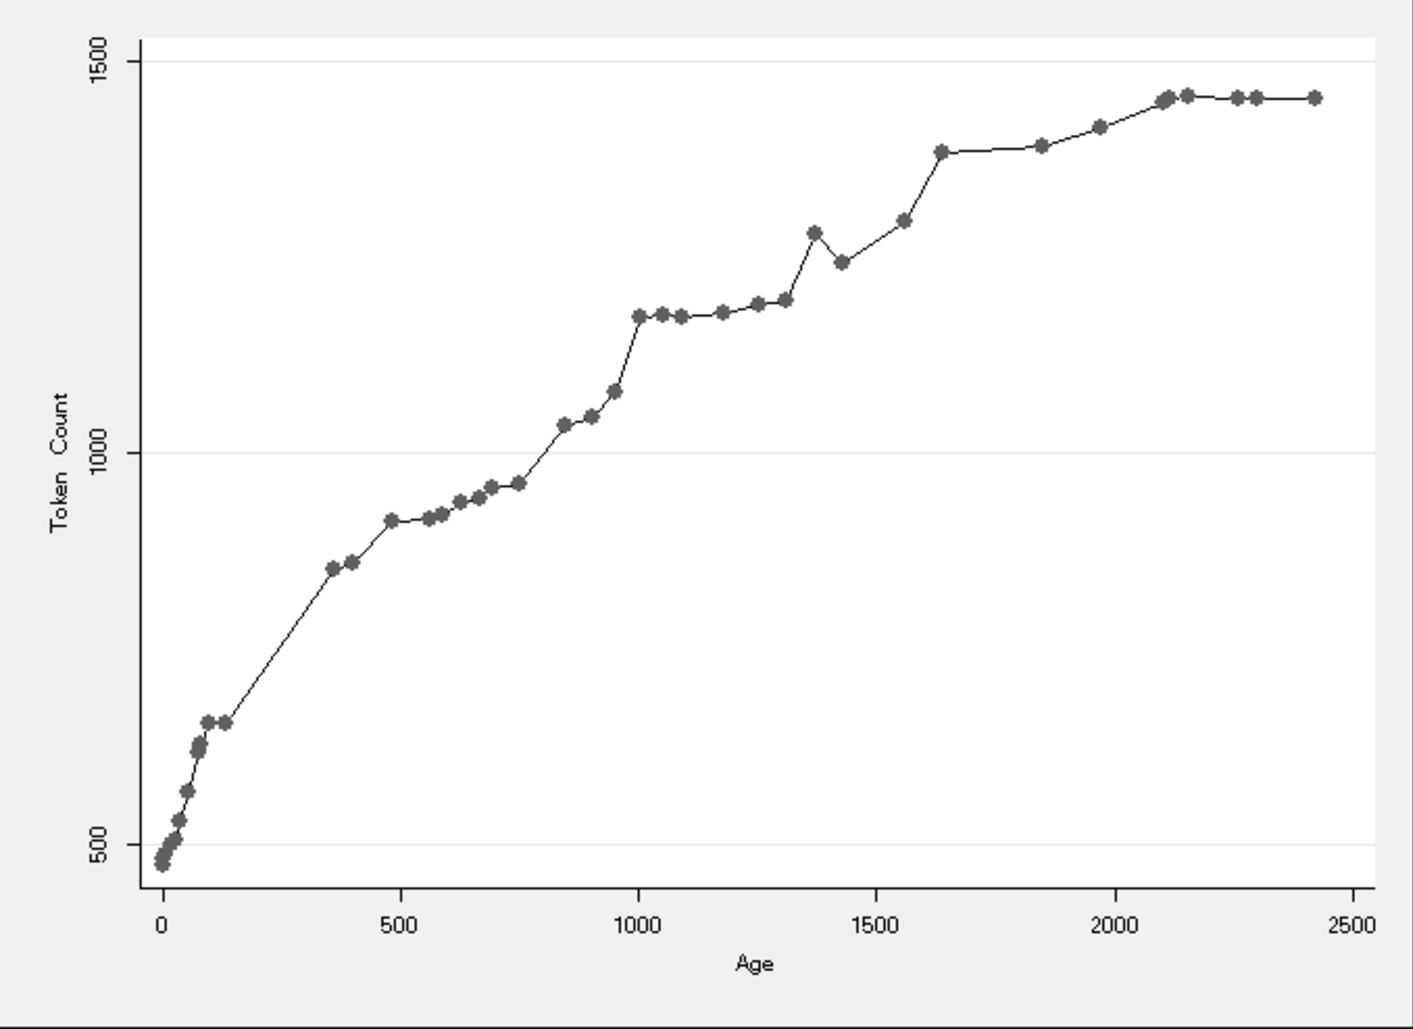
\includegraphics[width=\textwidth]{Figures/Vocab-PMDGrowth.pdf}
\caption{PMD vocabulary growth.}
\label{fig:vocab-growth-pmd}
\end{figure}

\textbf{Discussion}

Software system vocabularies appear to, in general, be reaching a level of maturity at a particular stage of their evolution, as shown by the results showing predominately sub-linear growth. This suggests, that the further growth of the software is being supported by core concepts that are already present within the vocabulary. However, in cases in which the vocabulary was showing growth that was not sub-linear, this was matched by a similar growth rate for system size. The implication of this is that new terms are being added to the vocabulary in order to support functional growth that is evident from the increase in system size.

Predictably, based on what we know of how software systems evolve, the growth of vocabulary is more substantial in earlier versions of software. This puts an emphasis on the need to devote efforts to documenting vocabulary for early releases. \textbf{Note: This alone is not enough to give an indication of when and what needs to be documented (e.g. some versions may exhibit smaller amounts of growth, but have a higher density of terms that have rich meaning within the vocabulary). However, the introduction of the number of terms that could potentially mean something is decreasing.}

\section{Distribution of Vocabulary} % (fold)
\label{sec:distribution_of_vocabulary}

\subsection{Measuring Distribution of Vocabulary} % (fold)
\label{sub:measuring_distribution_of_vocabulary}

\crumbs{Frequency distributions (to plot term usage distribution profile)}

\crumbs{Gini coefficient (to determine distribution of wealth amongst terms)}

% subsection measuring_distribution_of_vocabulary (end)

\subsection{Distribution Profiles} % (fold)
\label{sub:distribution_profiles}

\crumbs{Humans like to deal with a small number of abstractions, rather than lots. This is the case with software systems, where developers will extend the functionality of existing concepts, rather than build new ones (cite Raj's work, etc.).}

In this study, we investigated the how term usage within source code is distributed, to determine whether there is a tendency for developers to use a subset of the vocabulary with greater frequency than the rest of the vocabulary.

To determine how the vocabulary was distributed across the system, we plotted the frequency distribution for the number of occurrences for each term within the source code. We used a threshold value of 100 occurrences as a cut-off point to indicate that a term was used with an extremely high frequency.

\crumbs{Some summative statistics about the systems analysed}

\crumbs{Need to put some numbers in the following paragraph -- comparative \%s of number of terms over threshold of 100?}

\begin{figure}[t]
\centering
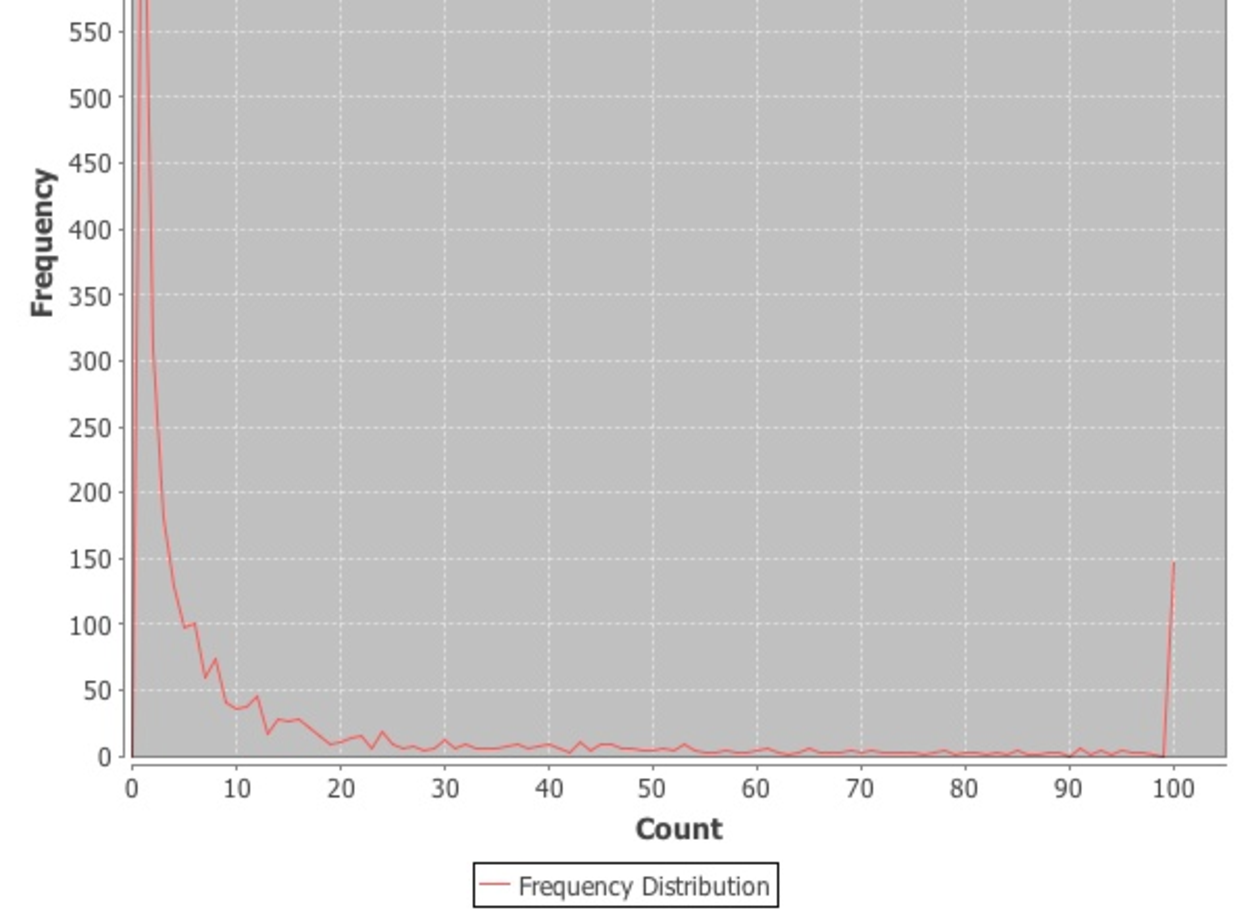
\includegraphics[width=\textwidth]{Figures/Vocab-GroovyFreqDist.pdf}
\caption{Groovy vocabulary frequency distribution.}
\label{fig:vocab-freq-dist-groovy}
\end{figure}

Each of the systems analysed exhibited a remarkably similar distribution. The tendency was towards the usage of a substantial proportion of terms less than 5 times throughout the source code. Further along the distribution profiles, a far smaller number of terms are used from 30-40 times. A small amount of terms were used in excess of the defined threshold value of 100.

Observing the frequency distribution across the entire history, one can observe \textbf{[How? Need some that demonstrates this clearly...have a version 1 and version n comparison?]} that a similar distribution profile is present from the initial versions of the software systems and is preserved as the system evolves. It is interesting to note, however, that the most noticeable trend in terms of changes to the distribution profile over time is the continual increase in the number of terms used only a very small number of times (1-5). The indication of this is that developers are not averse to the introduction of a lot of new terms, provided they will only be used a limited number of times. In contrast to this, there is also a consistent increase in the number of terms that exceed the occurrence threshold of 100. As the number of terms falling within the range of 5-99 occurrences demonstrates minor fluctuations over time, it appears that terms within this range, particularly towards the higher end, are being re-used in subsequent versions, causing the number of times they occur to exceed the threshold value of 100. The tendency of developers towards re-use of popular terms in discussed further in Section~\ref{sec:rich_get_richer}

\crumbs{The implications of this distribution profile is that terms that there is a predictable pattern as to how vocabulary are established within source code.}

\crumbs{Is there are similarity between NL distribution and source vocabulary distribution?}

% \crumbs{This is an indication that once terms become popular they are highly unlikely to lose much of their popularity and that how vocabularies are distributed seems to be unavoidable}

% \crumbs{Discuss why the vocabulary is consistently distributed in the same manner across systems}

% \crumbs{Discuss cases in which there are versions that match in Gini vs. Growth. Reason as to what this might be attributed to. Is it safe to say that in cases where there is this parallel, these versions are significant in terms of the vocabulary. What explanations may or may not support this reasoning?}

% subsection distribution_profiles (end)

% section distribution_of_vocabulary (end)

\section{Rich Get Richer} % (fold)
\label{sec:rich_get_richer}

Does the wealth of term usage within the vocabulary remain the same throughout evolution or do wealthy terms get continually richer as the software evolves?

Lehman's laws say familiarity will be conserved throughout evolution, which ensures the direction of the software is maintained based on what is familiar to those responsible for its development.

\crumbs{Important to preserve familiarity within vocabulary/source code as developers will change which pieces of code they will be working on...they need to ensure that terms are used consistently and re-used where appropriate}

% Vocabulary represents the most comprehensible aspect of the source code for developers. Therefore, it is important to preserve vocabulary that is part of concepts that make up the system.}

To determine whether developers favour the re-use of terms that are already popularly used, we examined how the distribution of wealth changes throughout evolution.

\crumbs{We investigated whether the distribution of vocabulary became more skewed over time (thus indicate term re-use and familiarity)}

\crumbs{Used the Gini coefficient to observe how wealth of term usage is distributed throughout the vocabulary}

"A low Gini coefficient indicates a relatively equal wealth distribution in a given population, with 0 denoting a perfectly equal wealth distribution (i.e., everybody has the same wealth). A high Gini coefficient, on the other hand, signifies a very uneven distribution of wealth, with a value of 1 signalling perfect inequality in which one in- dividual possesses all of the wealth in a given population." -- \textbf{Re-word and cite Raj's work using Gini here...}

Across of the systems, in each version, Gini values fall between 0.6-0.88. These figures generally increase in small amounts over time. An example typical change of Gini through evolution is shown for Groovy in Figure~\ref{fig:vocab-gini-groovy}. Rarely do Gini values change by a significant amount (> 4\%). Latest version values are all above 0.7 and in some cases ~0.85. This indicates that in some cases there are a small number of terms that continue to be re-used heavily, while an increasingly large number are hardly used at all. The bounded Gini values suggest that there is a limit to the amount that rich terms can be used and that the wealth of terms within the vocabulary must not be too concentrated.

\crumbs
{
Cover some of the more interesting Gini findings here:

- Only 13 systems demonstrated a decrease in Gini across versions that was above 0.01. Of those 13 systems, only 2 (Jetty and Tapestry) had a decrease that exceeded 0.04, a statistically signficant results.

Most increases in Gini were by far less than 0.04, however there were some exceptions to this:

ant: 0.06369188197063902 (2, 97)

axis: 0.06884638731906056 (23, 2555)

hsqldb: 0.05640940134193073 (21, 2839)

jetty: -0.04525546902999622 (13, 2681)

jetty: 0.04449631971116941 (17, 4184)

rssowl: 0.04789512032057741 (2, 168)

rssowl: 0.05992713617327339 (14, 2212)

tapestry: -0.04891624497153557 (13, 1576)

webwork: 0.05243274394700814 (10, 649)

\textbf{Should include some investigation here to indicate what has caused the relatively big changes...1-2 systems should do -- Jetty would likely be the most interesting, since it has a fairly big decrease, followed by an equally large increase}

}

\crumbs{Our findings indicate that the rich do get richer as a software system evolves. The high Gini values shown in more recent versions indicate that there are a small set of terms that are fundamental to the vocabulary present within the source code, and will inevitably be re-used. However, as these values seem to be bounded, we postulate that there are terms within the vocabulary that will see occasional heavy re-use, despite not being a core component of the vocabulary, which makes the richest terms relatively less wealthy.}

% \crumbs{It seems inevitable that the rich terms will be continually used. This means that choosing the right terms (consistent and comprehensible) to become rich is important, as they will only gain greater momentum as time goes on.}

\begin{figure}[t]
\centering
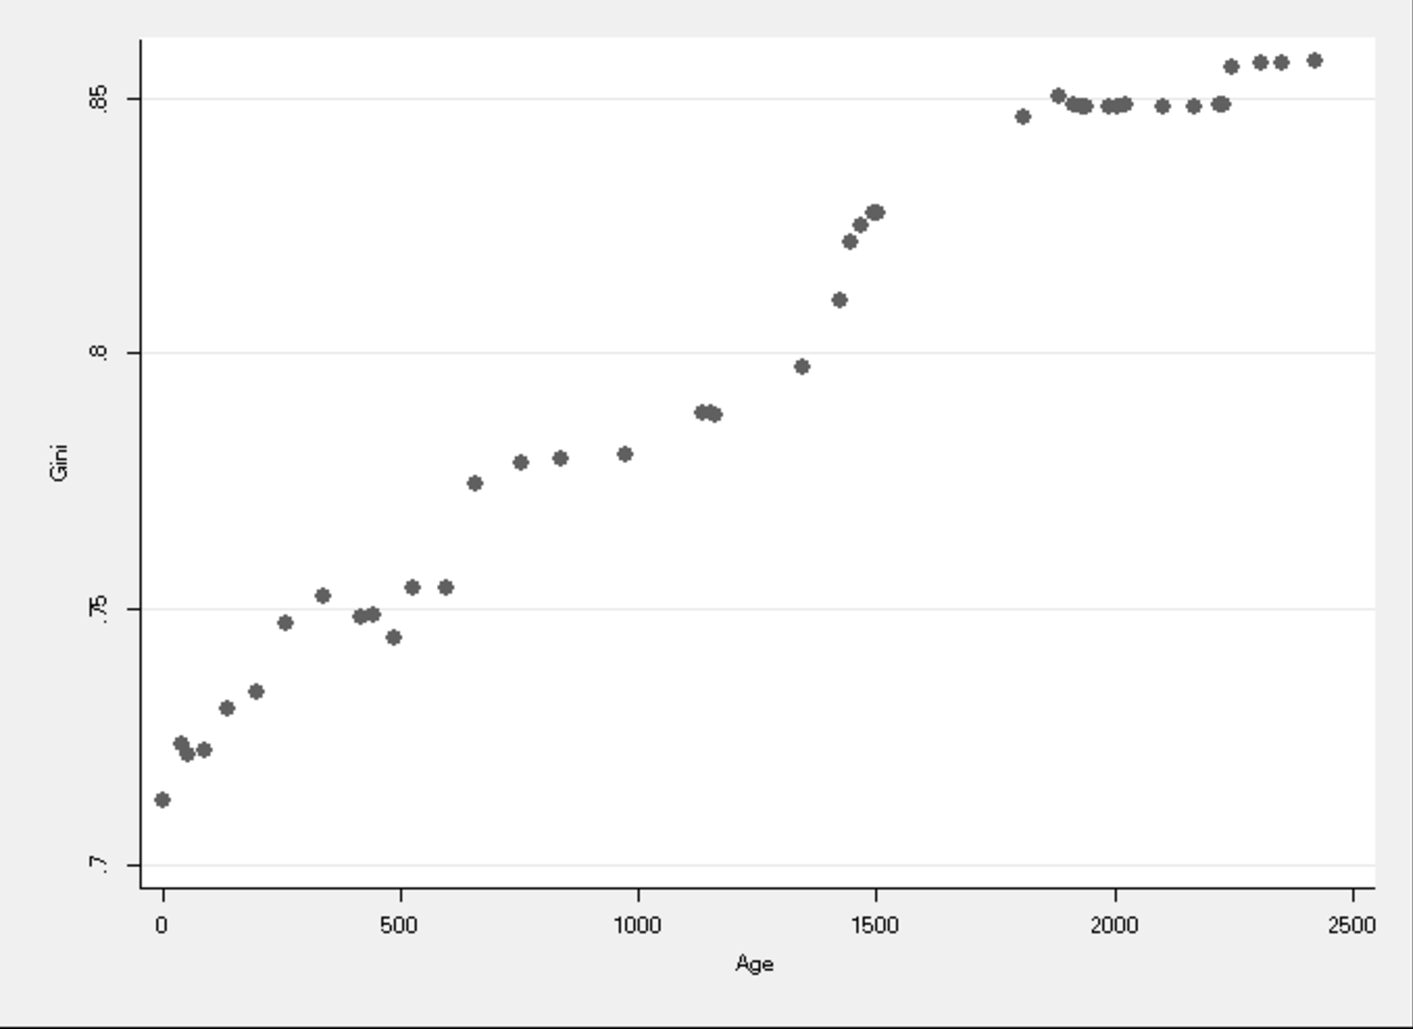
\includegraphics[width=\textwidth]{Figures/Vocab-GroovyGini.pdf}
\caption{Groovy term Gini.}
\label{fig:vocab-gini-groovy}
\end{figure}

% section rich_get_richer (end)

\section{Frequency vs. Age} % (fold)
\label{sec:frequency_vs_age}

Does the age of a term have an influence on the likelihood is used? Do new features being introduced result in new supporting vocabulary that is used heavily or is there a tendency to re-use vocabulary that is already there?

\crumbs{Investigated whether there is a correlation between the age of a term and it's likelihood for re-use}

\crumbs{Implications of correlation (or inverse, or lack thereof) -- table}

\crumbs{Found that there were more older terms that were used most frequently, but that a few had been introduced along the way and seen a good amount of usage.}

\begin{figure}[t]
\centering
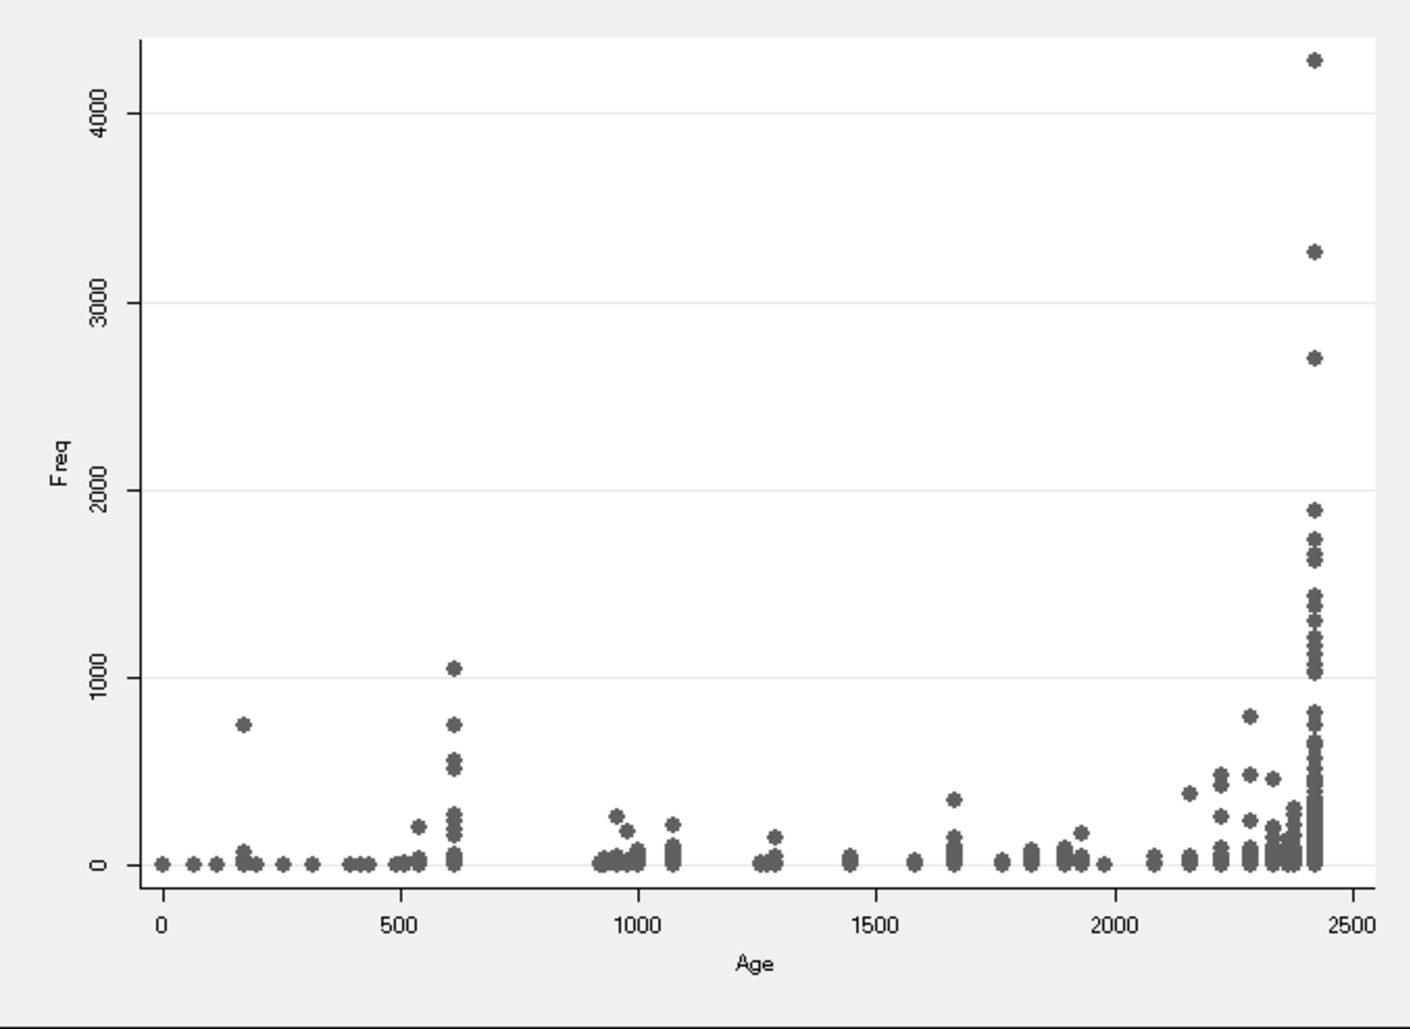
\includegraphics[width=\textwidth]{Figures/Vocab-GroovyFrequencyAge.pdf}
\caption{Groovy vocabulary freq-age scatter.}
\label{fig:vocab-freqage-groovy}
\end{figure}

\crumbs{\textbf{Histogram}}

\crumbs
{
Findings are that some systems demonstrate a stronger correlation between the age of a term and it's likelihood of being re-used

\textbf{What is causing this?}

\textbf{Include results from Raj's analysis here}
}

This indicates that vocabulary is not entirely established from the start and that new terms can be introduced and used heavily. This highlights the importance of watching for big changes in vocabulary as time goes on to ensure that new concepts are identified and dealt with appropriately. While the very core concepts are maintained, there are clearly important elements of the vocabulary introduced over time, important enough to warrant some attention.

Likely an importance and re-usability based on the role of the term within the vocabulary. Some terms introduced early are introduced with lower significance than other terms and, accordingly, are subject to lesser or no re-use.

% section frequency_vs_age (end)

\section{Mining the Domain Model} % (fold)
\label{sec:mining_the_domain_model}

What do the most frequently used terms within vocabularies refer to? Are they primarily pertaining to the software's domain, its design elements or something entirely different?

Best practices in software development suggest that programmers will write code that is communicative of the purpose and intention of the software system. When practising object-oriented programming, there are general guidelines that suggest how developers should reason about the design of their application, which allows them to build a solution around the problem they are trying to solve. These guidelines include the usage of a domain model, which captures the main entities within the problem space, as well as design patterns and idioms that represent re-usable concepts that can be applied to tailoring a system's architecture to suit the problem.

While these guidelines are in place to aid developers in the design and implementation of their applications, there is no governance with regard to how developers apply the vocabulary associated with them within their source code. While we can speculate that developers make use of domain related terms, it is uncertain as to whether developers actually utilise the vocabulary associated with these guidelines to good effect when writing code.

To determine whether developers effectively use domain-related terms within their source code's vocabulary, we extracted the 15 most popular terms from the latest version of each of the systems.

\subsection{Case Studies} % (fold)
\label{sub:case_studies}

\subsubsection{Hibernate} % (fold)
\label{ssub:hibernate}

\crumbs{Composed of \emph{n} terms overall.}

\begin{figure}[t]
\centering
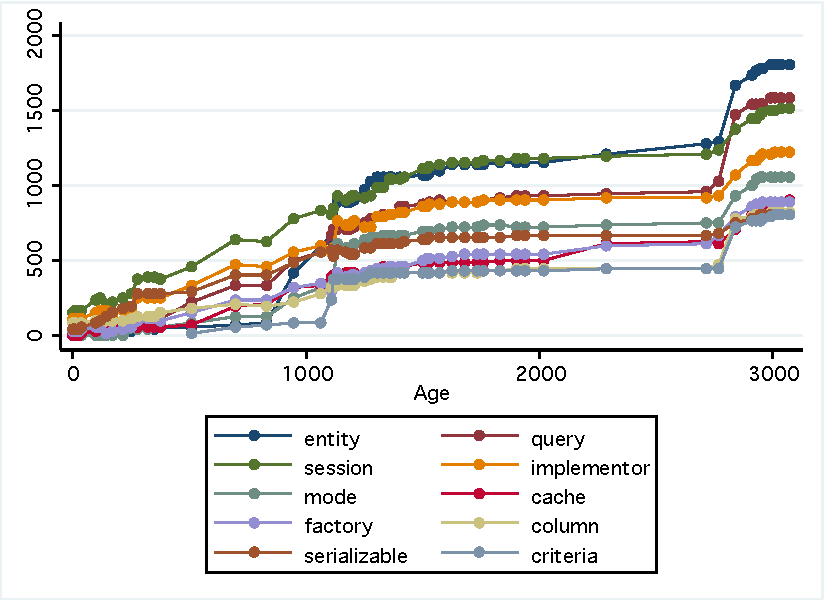
\includegraphics[width=\textwidth]{Figures/Vocab-HibernatePopular.pdf}
\caption{Hibernate most popular terms.}
\label{fig:vocab-popular-terms-hibernate}
\end{figure}

\crumbs{x of the most popular terms refer to domain-related concepts}

\crumbs{Comment on the usage of popular terms over time...highlight any terms that were introduced in later versions or those that were less popular and gained substantial popularity to become the most popular.}

% subsubsection hibernate (end)

\subsubsection{Struts} % (fold)
\label{ssub:struts}

\crumbs{Composed of \emph{n} terms overall.}

\begin{figure}[t]
\centering
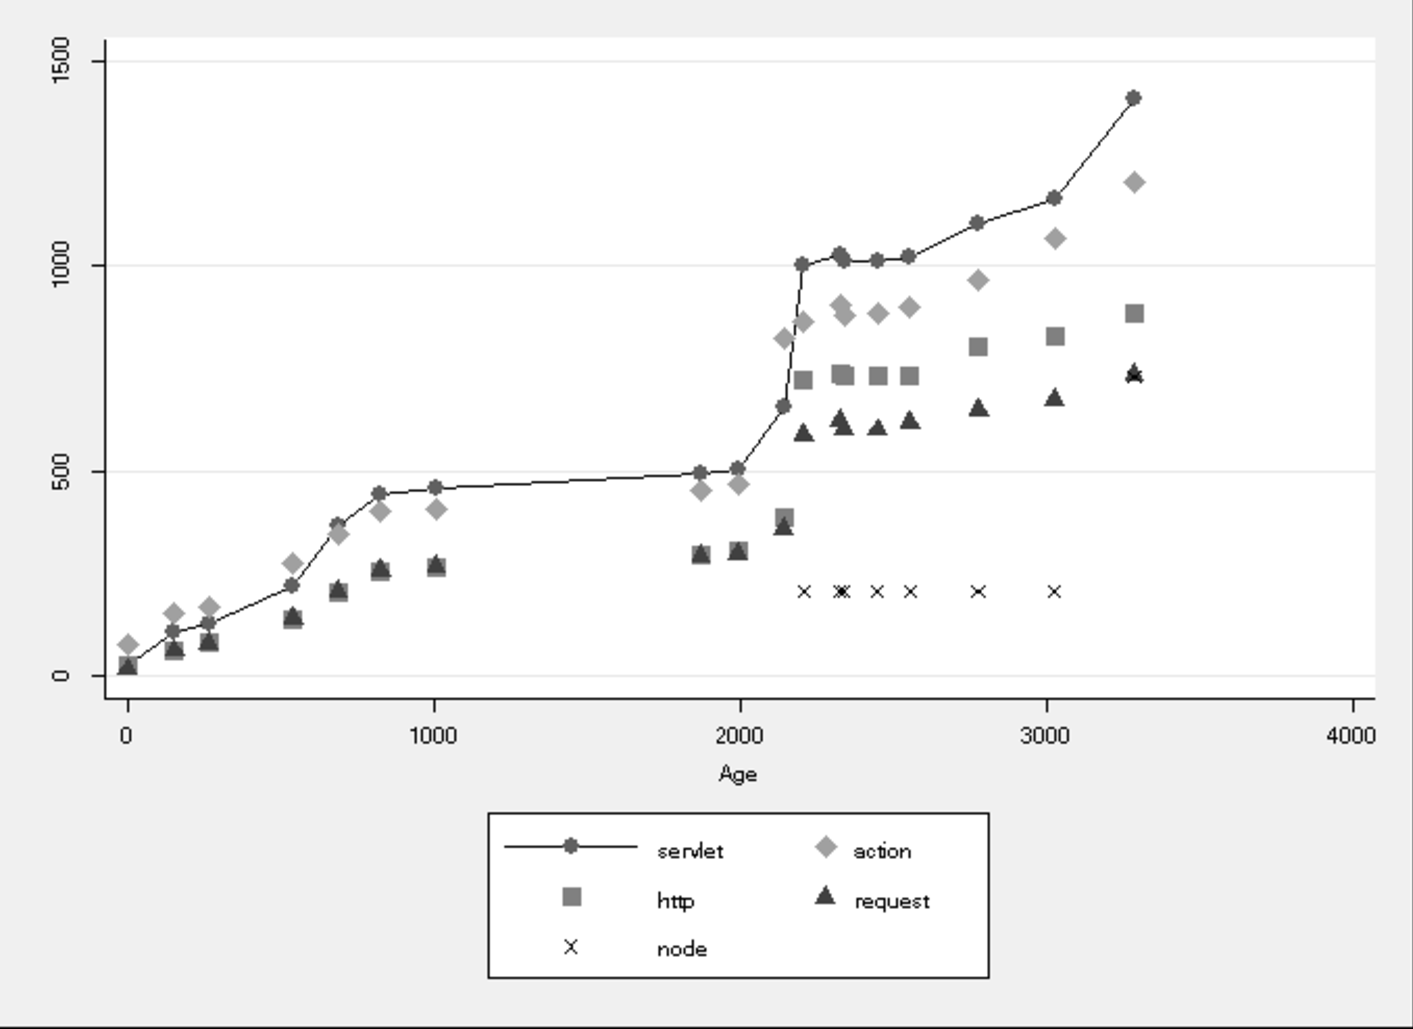
\includegraphics[width=\textwidth]{Figures/Vocab-StrutsPopular.pdf}
\caption{Struts most popular terms.}
\label{fig:vocab-popular-terms-struts}
\end{figure}

\crumbs{x of the most popular terms refer to domain-related concepts}

\crumbs{Comment on the usage of popular terms over time...highlight any terms that were introduced in later versions or those that were less popular and gained substantial popularity to become the most popular.}

% subsubsection struts (end)

\subsubsection{Avasa} % (fold)
\label{ssub:avasa}

\crumbs{Composed of \emph{n} terms overall.}

\begin{figure}[t]
\centering
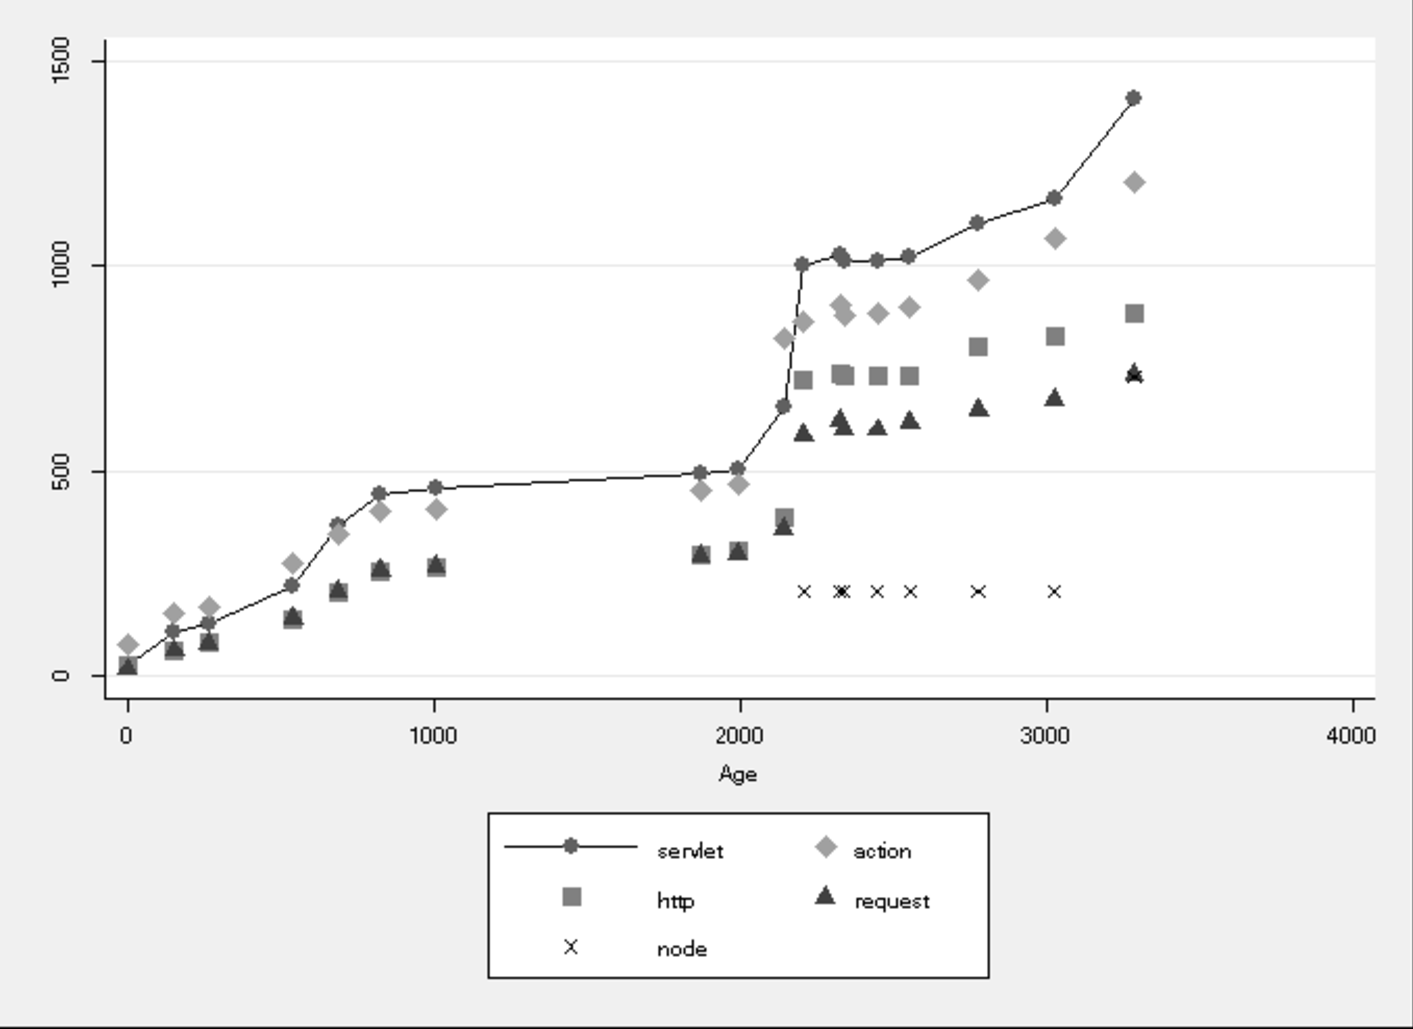
\includegraphics[width=\textwidth]{Figures/Vocab-StrutsPopular.pdf}
\caption{Struts most popular terms.}
\label{fig:vocab-popular-terms-struts}
\end{figure}

\crumbs{x of the most popular terms refer to domain-related concepts}

\crumbs{Comment on the usage of popular terms over time...highlight any terms that were introduced in later versions or those that were less popular and gained substantial popularity to become the most popular.}

% subsubsection avasa (end)

% subsection case_studies (end)

\crumbs{Implications of this is that the domain model entities are well-represented within source code -- this is encouraging...indicates that developers favour heavy usage of the most conceptually rich terms within their source code}

Interestingly, the usage of the most popular terms does not seem to increase at a constant rate across all versions. The results indicate that the usage of a term is more likely to increase in small bursts across separate versions. We postulate that this may coincide with versions in which more substantial change is occurring, which is reflected by relatively large increase in the usage of popular terms. In versions in which this is not the case, we suggest that more localised changes are occurring (i.e. changes that occur within existing classes and methods, that would not result in an increase in the number of classes, methods or fields which are the level of abstractions for which we consider terms to be contributing towards the vocabulary).

% section mining_the_domain_model (end)

% chapter findings (end)